\documentclass{article}
\usepackage[utf8]{inputenc}
%\usepackage{cite}
\usepackage{graphicx}
\usepackage{listings}
\usepackage{url}
\usepackage[normalem]{ulem}
\useunder{\uline}{\ul}{}
%\usepackage{minted}

\title{GDMA Project: \\ CDDB as Graph Database}
\author{Julian Schelb (1069967)}
\date{June 2022}

\newcommand{\name}[1]{\texttt{\emph{#1}}}

\begin{document}

\maketitle

\section{Importing Data}

This chapter describes design decisions made to map the relational CDDB database to a graph database. See Jupyter notebook \path{01_Import_Data.ipynb}.

\begin{figure}[ht]
    \centering
    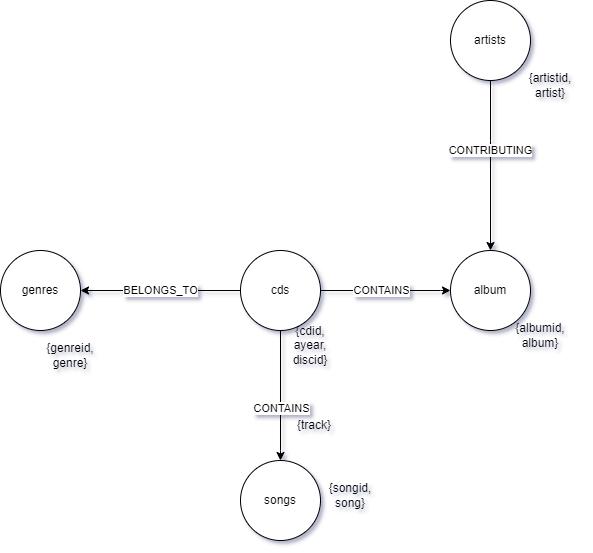
\includegraphics[width=11.5cm]{../Figures/cddb_as_graph-Default.png}
    \caption{CDDB Graph Schema }
\end{figure}

\subsection{Mappping of Tables}
Entries in tables \name{artists}, \name{albums}, \name{songs} and \name{cds} represent entities and are mapped to nodes of appropriate type. The cross table  \name{cdtracks} is mapped as relations between CDs and Songs with the property \name{track}. The cross table  \name{artist2album} is mapped as a triangular relationships, using six relations each to connect Artists, Albums and CDs in both directions.

\subsection{Bidirectional Relations}

To consgtruct the queries necessary for subsequent tasks, it was structly speaking not necessary to create relations for both directions. However, doing so allows for more readable queries. In addition, the relational SQL database does not define a direction for relations either, and this property is thereby preserved.

\subsection{Unique Identifiers}
The unique identifiers present in the SQL database are preserved as node properties. Although Neo4j automatically assigns different IDs internally, this preserves compatibility with the SQL version. It is conceivable that in the real worlds, queries may reference those IDs directly. For example as hardcoded list as part of a GUI.

\subsection{Entity Names}
As in the SQL version, the actual name of a \name{song}, \name{genre}, \name{album} and \name{artist} is a property named after the entity type and therefore different per node label. This was done to map the SQL version as closely as possible to the graph version. In real world scenarios it may be beneficial to rename these properties to \name{name} across all nodes. This would allow for simpler queries in cases where nodes of different types are filtered by name. Also, a joint full-text index would be possible.

\subsection{Indices}
To speed up \texttt{MERGE} and \texttt{MATCH} operations, the IDs for nodes with label \name{Artist}, \name{Album}, \name{Genre}, \name{Song} or \name{CD} are indexed. In addition, a full text index is used for the names of \name{Artists}, \name{Albums} and \name{Songs} to allow for imprecise searches (fuzzy search).

\subsection{Importing Songs}

Songs with a trailing backslashcoused problems because the closing quote is escaped. To mitigate this, an extra whitespace character is added to those song titles. Effected rows can be found with the following sql statement:


\begin{lstlisting}[language=sql]
    SELECT * 
    from cddb.songs s 
    where song like '%\\' 
      and song not like '%\\\\'
\end{lstlisting}

Statement to update the rows:

\begin{lstlisting}[language=sql]
    UPDATE cddb.songs 
    SET song = song || ' ' 
    WHERE song LIKE '%\\' 
      AND song NOT LIKE '%\\\\'
\end{lstlisting}


% Lorem Ipsum ... ~\cite{Nobody06}.

\section{Cypher Queries}

See Jupyter notebook \path{02_Cypher_Queries.ipynb}.

\section{SQL to Cypher}

See Jupyter notebook \path{03_SQL_to_Cypher.ipynb}.

\section{Searching and Ranking}

See Jupyter notebook \path{04_Searching_and_Ranking.ipynb}.

\subsection{Search Implementation Details}

\vspace*{0.1cm}

\noindent
The search accepts a user supplied query string and returns an ordered list of the most relevant CDs. Three features are considered to rank CDs by relevance: Text similarity with the query string, user-preferred CDs and user-preferred genres. Since the user's preference is known prior to searching, the corresponding preference scores can be computed in advance. This leads to a two stage process:


\subsubsection{Stage 1: Precompute User Preference}

\noindent
Preferred CDs and genres are determined based on content previously liked by the user. To find preferred CDs, a subgraph of artists, albums and songs liked by the user and associated CDs is extracted. Subsequently, a centrality score is calculated for each node in both. The basic idea is that the most relevant CDs will have a high centrality score. To determine the preferred genres, we count how often genres are associated with the user's liked nodes. The basic idea is that the user prefers content of a few genres and therefore likes many albums, artists and songs belonging to those genres.

%\vspace*{0.5cm}
\newpage

\subsubsection{Stage 2: Search based on User Input}
\noindent
The most significant feature is the text similarity to the search query provided by the user. By using "Full-Text Indices" of Neo4J, the text similarity between artist name, album title and song title is calculated. The similarity score of all nodes associated with a CD are aggregated and used as a "Content Match Score".

\begin{equation}
    S_{Combined}= S_{Content} + (S_{CD}  * S_{Content} ) + (S_{Genre} * S_{Content} )
\end{equation}

\vspace*{0.5cm}

\noindent
The "Content Match Score" is then combined with the previously computed user specific "CD Preference Score" and "Genre Preference Score". The ten CDs with the highest combined score are presented to the user.



\begin{figure}[ht]
    \centering
    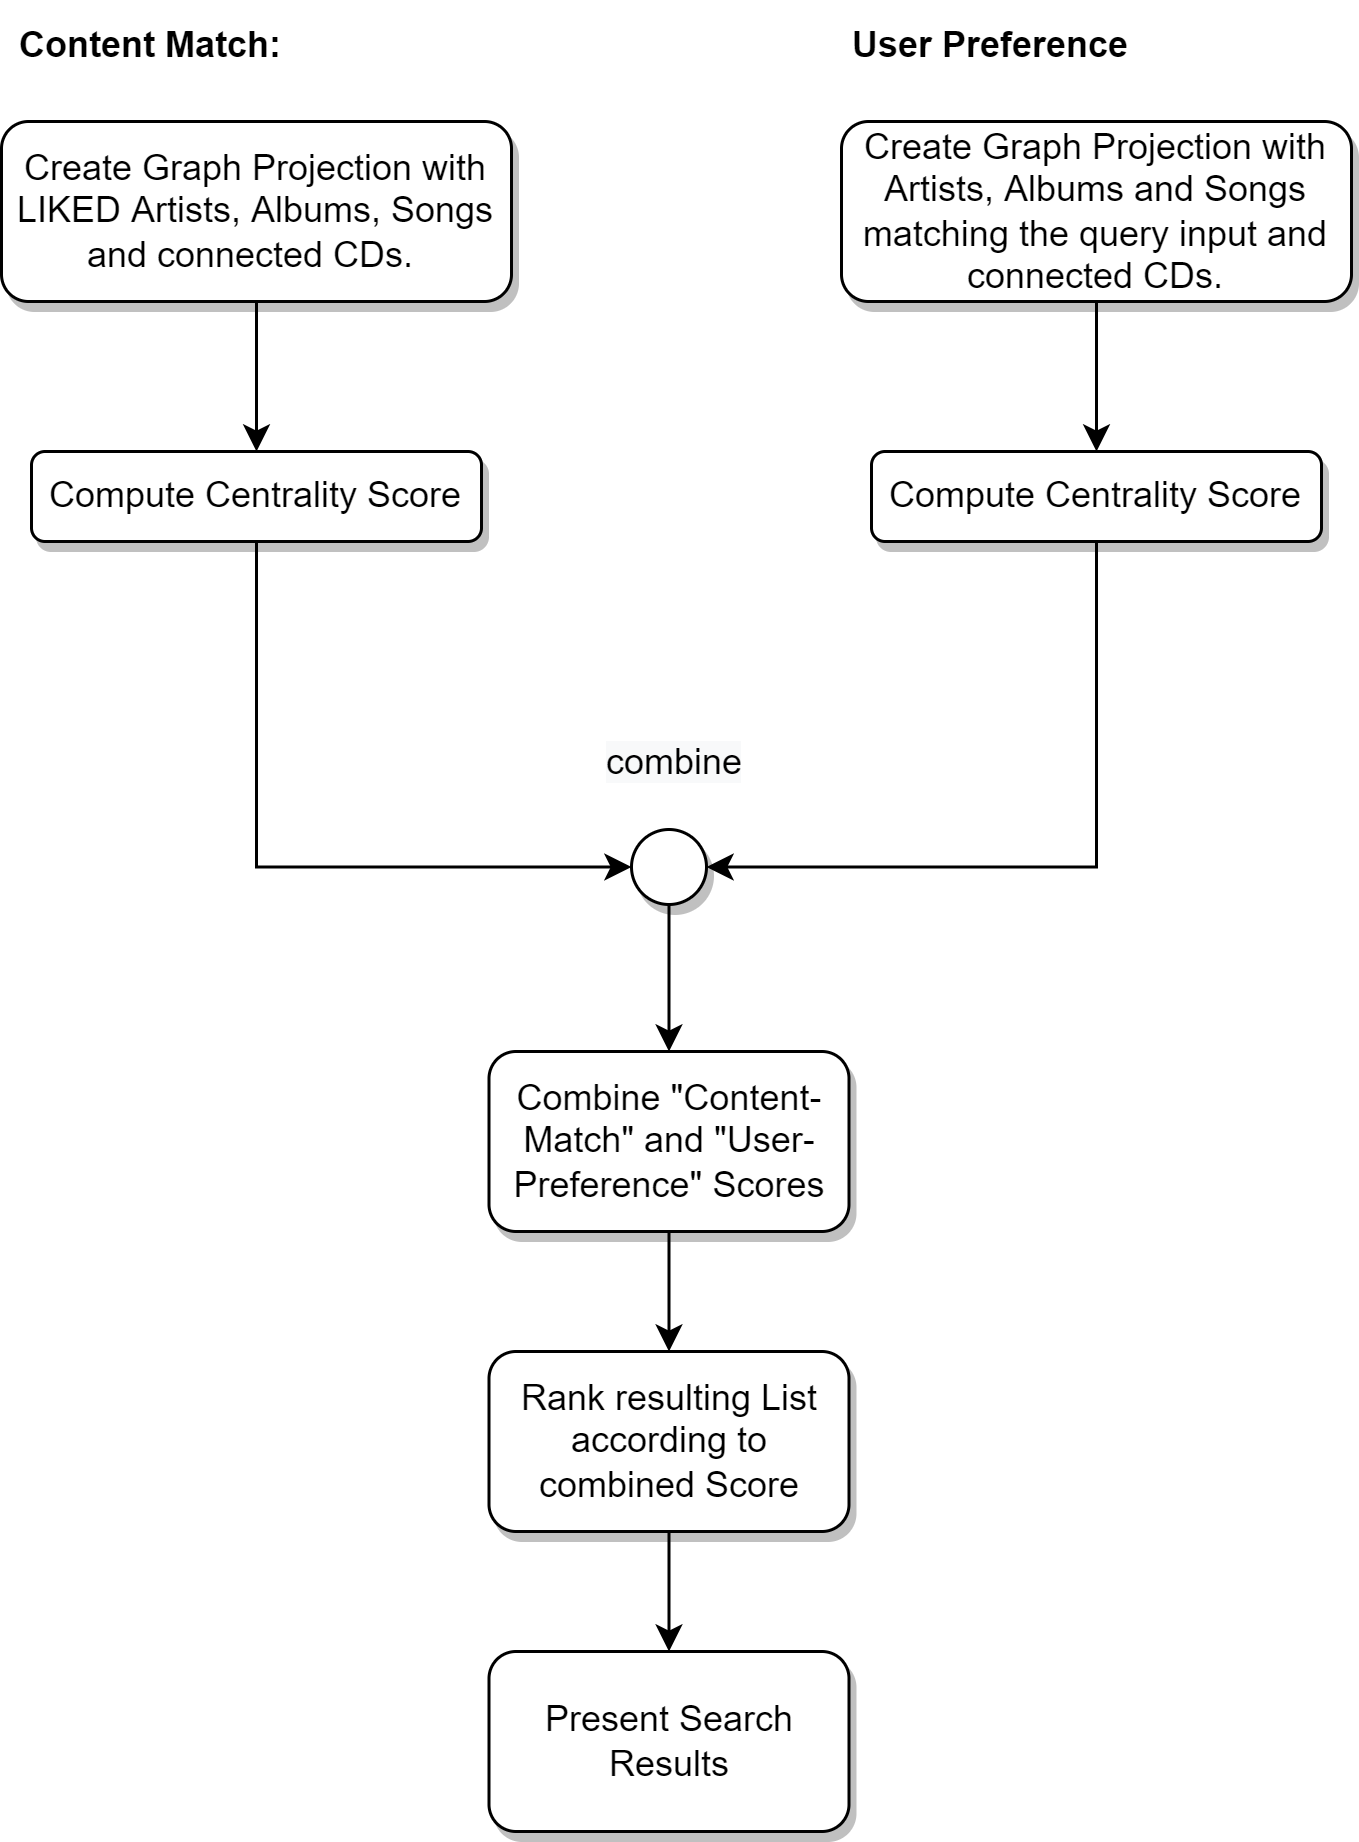
\includegraphics[width=11.5cm]{../Figures/search.png}
    \caption{Two stage process of calculating a CD relevance score by using text similarity and user preference as features.}
\end{figure}

\subsection{Example Search Queries}

The following example demonstrates how user 1 is searching for CDs related to "Jimmi Hendrix."
See Jupyter notebook \path{05_Search_Demonstration.ipynb} for more detailed examples.

\lstset{
    language=Python,
    showstringspaces=false,
    formfeed=\newpage,
    tabsize=4,
    commentstyle=\itshape,
    basicstyle=\ttfamily\footnotesize,
    morekeywords={models, lambda, forms},
}

\begin{lstlisting}

    # User specified search query
    search_input = "Jimi Hendrix purple haze are you experienced"
    user_id = 1
    search_mask = "all"

    # Search for relevant CDs
    searchFor(driver, database_name = "cddb", 
              user_id, search_input, search_mask)
\end{lstlisting}

\begin{table}[!htbp]
    \begin{tabular}{rr|rrrr|rr|}
        \cline{3-8}
        \multicolumn{1}{l}{} & \multicolumn{1}{l|}{} & \multicolumn{4}{c|}{\textbf{Score}}   & \multicolumn{2}{c|}{\textbf{CD Details}}                                                                                                                            \\ \hline
        \textbf{}            & \textbf{ID}           & \multicolumn{1}{r|}{\textbf{Content}} & \multicolumn{1}{r|}{\textbf{CD}}         & \multicolumn{1}{r|}{\textbf{Genre}} & {\ul \textbf{Comb.}} & \multicolumn{1}{r|}{\textbf{Genre}} & \textbf{Artists}      \\ \hline
        \textbf{0}           & 677                   & 31.53                                 & 0.5663                                   & 0.6632                              & \textbf{70.31}       & {[}rock{]}                          & {[}jimi hendrix{]}    \\
        \textbf{1}           & 35734                 & 31.53                                 & 0.5541                                   & 0.6632                              & \textbf{69.93}       & {[}rock{]}                          & {[}jimi hendrix{]}    \\
        \textbf{2}           & 136907                & 31.53                                 & 0.5541                                   & 0.6632                              & \textbf{69.93}       & {[}rock{]}                          & {[}jimi hendrix{]}    \\
        \textbf{3}           & 46232                 & 26.72                                 & 0.6927                                   & 0.6632                              & \textbf{62.96}       & {[}rock{]}                          & {[}jimi hendrix{]}    \\
        \textbf{4}           & 162186                & 26.72                                 & 0.6581                                   & 0.6632                              & \textbf{62.03}       & {[}rock{]}                          & {[}jimi hendrix{]}    \\
        \textbf{5}           & 7923                  & 56.69                                 & 0.0000                                   & 0.0714                              & \textbf{60.73}       & {[}blues{]}                         & {[}signature licks{]} \\
        \textbf{6}           & 1936                  & 24.34                                 & 0.6927                                   & 0.6632                              & \textbf{57.35}       & {[}rock{]}                          & {[}jimi hendrix{]}    \\
        \textbf{7}           & 33321                 & 28.27                                 & 0.2123                                   & 0.6632                              & \textbf{53.03}       & {[}rock{]}                          & {[}jimi hendrix{]}    \\
        \textbf{8}           & 2023                  & 26.72                                 & 0.6927                                   & 0.0714                              & \textbf{47.14}       & {[}blues{]}                         & {[}jimi hendrix{]}    \\
        \textbf{9}           & 17266                 & 20.76                                 & 0.3463                                   & 0.6632                              & \textbf{41.73}       & {[}rock{]}                          & {[}jimi hendrix{]}    \\ \hline
    \end{tabular}
\end{table}
% \bibliography{references}{}
% \bibliographystyle{plain}
\end{document}
